\chapter{Scepia}\thumbforchapter
\chapterauthor{Rebecca R. Snabel*, Maarten van der Sande*, Gert Jan Veenstra, Simon J. van Heeringen}
\newpage

\section{Introduction}

The state of a cell's gene activity is shaped by a complex network of genes and proteins, including transcription factors (TFs). TFs interact with the DNA by binding to it and changing the chromatin state or interacting with other transcription factors. 

Single-cell transcriptomics has emerged as a rapidly expanding field, allowing researchers to explore the gene expression profiles of diverse cell types with increasing ease and affordability. However, when it comes to examining chromatin accessibility or histone context, crucial aspects of gene regulation, challenges persist. Single-cell ATAC-seq (scATAC), while immensely valuable, remains relatively costly and generates sparser data compared to transcriptomic methods. Single-cell ChIP? Even more recently single cell CUT\&Tag (scCUT\&Tag) a method able to measure histone modifications as well as transcription factor chromatin occupancies on a single-cell level, was established. 
Consequently, many laboratories encounter difficulties in adopting these techniques due to budget constraints and resource limitations...



Do we mention scenic in the introduction? 

Large databases already exist with lots of chromatin accessibility and histone modification chip seq data. For example SRA, but also more standardized projects such as ENCODE and REMAP. These databases serve as great starting point for explorative analyses. But in addition, as the relationship between different genomic marks and transcriptomic data is redundant(more refs \cite{Wang2016}), this also begs the question whether it is necessary to perform single-cell chip/atac in addition to single-cell RNA-seq. An example is regulatory potential. Wang \textit{et al.} calculate h3k27ac regulatory potential. Regulatory potential is curve. The regulatory potential in turn could predict which genes were downregulated after exposure to BET inhibitors.

To answer this question we developed a tool for Single-Cell Epigenome-based Inference of Activity (scepia). Scepia matches single-cell RNA-seq data to a reference database of H3K27ac signal through regulatory potential. On this reference database then motif scanning. To test the performance we test on HHCA v2. 

Why HHCA (v2) -> Multiome. Interest in Heart specifically?

To \textit{test} how SCEPIA performs on real data, we have used the latest version of the human Heart Cell Atlas v2 (REF XXX HHCA v1, HHCA v2). The version 2 of this dataset additionally consists of single-cell chromatin accessibility data alongside transcriptomic data from the same nuclei, by combining both versions of the atlas the authors produced an extensive atlas covering the different tissues and cellular subtypes present in the human adult heart. A lot is known about different cellular markers and regulators of the different cell types within the heart, however, much can also still be gained from more detailed research on further epigenetic regulation within the heart, and the transcriptional actors contributing to this. However, in this research only the openness of the chromatin is captured, not the more detailed information on the histone modification differences, which can inform on whether an accessible region acts as an active enhancer. Cardio-vascular diseases are still the number one cause of deaths worldwide (\href{https://doi.org/10.1161/CIR.0000000000001123}{https://doi.org/10.1161/CIR.0000000000001123}), and the ability to research intricate differences between healthy and diseased tissues in a multimodal setting, will help to gain more understanding of the complex (dis)regulation happening in these tissues, also on the less researched field of epigenetic on a cellular//cell type level. 

\textit{The availability of the single-cell chromatin accessibility data, can be used as a epigentic read-out for and thereby brings us one step closer to the type of data SCEPIA will infer. This allows us to validate the performance of our tool in predicting epigenetic/transcriptional regulation from a single-cell transcriptomic dataset. // SCEPIA infers per single cell the active enhancer signal from public ChIP-seq data resources, although accessibility of the chromatin is one read-out of the effect of such active enhancer signal.}

\section{Results}

\subsection{Matching regulatory potential and transcripts}

We hypothesized that incorporating a measure of cis-regulatory element activity, such as ATAC-seq or H3K27ac ChIP-seq, would be beneficial to identify transcription factor motif activity from single cell RNA-seq data, even when this is not experimentally measured. Here, we used the \textit{regulatory potential} to match single cell RNA-seq profiles to a database of known H3K27ac ChIP-seq profiles. The regulatory potential is defined as the weighted average H3K27ac signal per gene \cite{Wang2016}.  To determine how well the  regulatory potential specifically matches the RNA-seq data for identical (or similar) cell types , we obtained data from 96 human RNA-seq cell types and 121 human H3K27ac cell types from ENCODE\cite{encode_dcc}  (Supplementary Table SX). We calculated the regulatory potential for all H3K27ac samples (see Methods). We then computed the correlation coefficient for all possible combinations of regulatory potential and RNA-seq values (Fig. \ref{fig:bulk_comparison}). In general the regulatory potential shows only  a high positive correlation for a subset of the RNA-seq, indicating that measure captues a cell type-specific signal. The average correlation coefficient for matching cell types between regulatory potential and transcripts per million (TPM) was found to be $0.53 \pm 0.14$. In 64\% of instances, the regulatory potential of a given tissue exhibited the highest correlation with the TPM of the same tissue. Furthermore, in 77\% of the cases, the highest correlation was observed with a tissue sharing the same ontology term. As noted previously \cite{Wang2016},  the specific parameters used for calculating regulatory potential do not significantly impact the results. For this specific analysis, the H3K27ac signal in the promoter region alone is sufficient to predict the TPM. In summary, our findings suggest that a database of H3K27ac regulatory potential can effectively serve as a reliable classifier for characterizing cell states based on transcriptomic data.

\begin{figure}
    \centering
    \includegraphics[width=1\linewidth]{ch.scepia/imgs/celltypes.png}
    \caption{\textbf{Regulatory potential is a good predictor for H3K27ac cell state.} \textbf{(A)}: The Pearson correlation coefficients between all combinations of 121 H3K27ac regulatory potentials and 96 RNA TPMs. Highlighted are XYZ bla bla. \textbf{(B)}: bla bla. How to call subset?}
    \label{fig:bulk_comparison}
\end{figure}

In general H3K27ac signal can be used to determine motif or transcription factor activity, as described previously (refs). This score/measure, which quantifies the contribution of each motif to H327ac peak strength, has been shown to be a powerful measure of the relevance of a transcription factor for a specific cell state. The relationship between RNA-seq and regulatory potential led us to assume that transcription factor motif activity can be inferred from transcriptomic data, through an intermediate of matched H3K27ac data. To investigate this, we tested how well the transcription factor activity inferred from RNA-seq matches the transcription factor activity determined directly from H3K27ac. As the reference database contains a limited number of cell types, an exact matching cell type may not be available for a specific cell type measured by RNA-seq. Therefore, we decided to calculate a composite measure of motif activity, based on a combination of reference cell types. To calculate this measure, we regressed the TPM values of the 2,000 most variable genes of a collection of cell  types against our regulatory potential database. From there, we selected the top 50 cell types based on the absolute regression coefficients and identified the top 10,000 most differentially enriched cis-regulatory regions within these 50 cell types. Subsequently, we calculated the motif activity using these enhancers, and obtained the final motif scores by taking the dot product of motif scores and regression coefficients. To test our composite activity score, we made one hundred random subsets of five tissues common to both our H3K27ac reference database and transcriptomic dataset. Our first step involved establishing a ground truth for motif activities by conducting a motif scan on the top 25,000 most differentially enriched enhancers within each of these five tissues. Here, enhancers were defined as peaks within the REMAP dataset located more than 2kb away from the transcription start site. A naive approach to estimating motif activity based solely on transcriptomic data would assume a direct one-to-one translation between the transcripts per million (TPM) values of a transcription factor and its motif score. However, as Figure \ref{fig:bulk_comparison}B illustrates, this naive approach displayed a poor correlation with our ground truth data. Instead,  the more sophisticated approach based on regulatory potential demonstrates a significantly improved correlation compared to the naive method (refer to Figure \ref{fig:bulk_benchmark}B). Finally, to assess the sensitivity of our approach to the choice of enhancer set, we compared the ground truth data based on the top 25,000 most variable enhancers with that based on the top 10,000 most variable enhancers.
Taken together, these analyses show that RNA-seq can be matched to H3K27ac in a cell type-specific manner, and that this data can be used to estimate transcription factor activity. <implication for single cell RNA-seq> 
See supplemental figure XXX for parameter sweep. This is nice because test/validate separate

\subsection{Single-Cell Epigenome-based Inference of Activity}

Single-cell has the advantage of multiple measurements so significance tests.

\begin{figure}
    \centering
    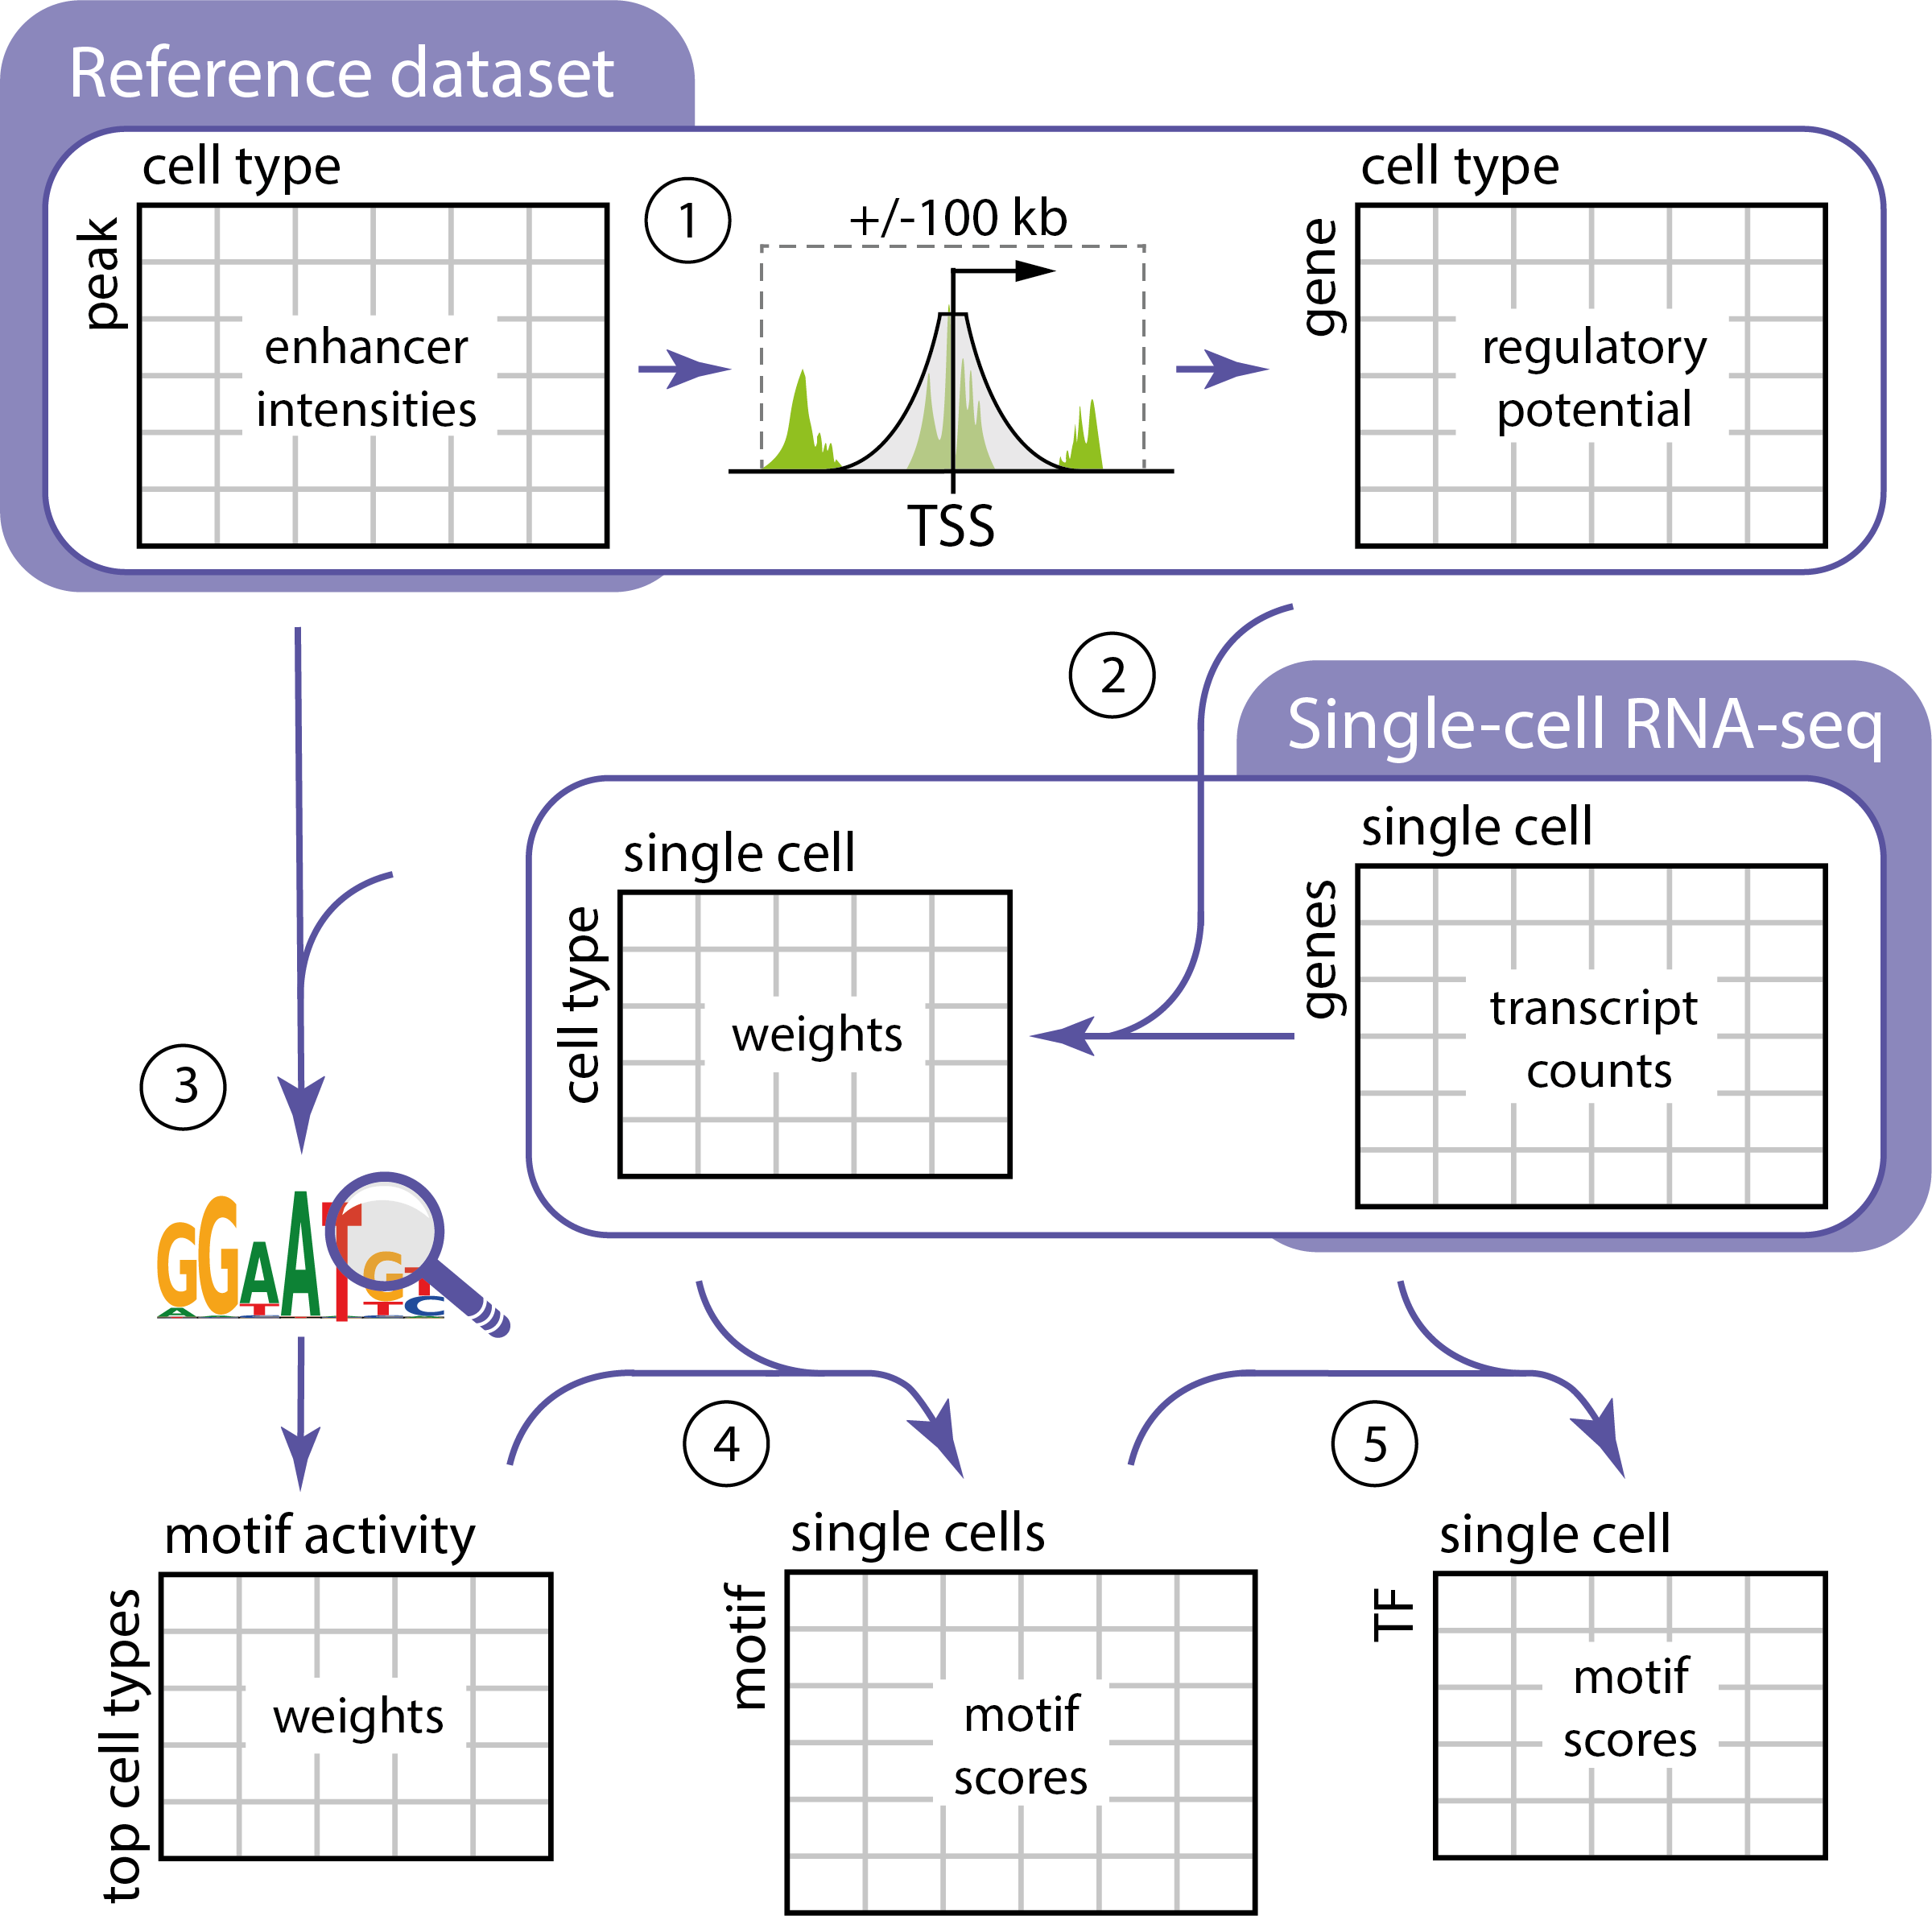
\includegraphics[width=1\linewidth]{20231106_OverviewFigure_SvH_v2.png}
    \caption{\textbf{Figure XX: Scepia matches X Y Z}, TODO}
    \label{fig:scepia_overview}
\end{figure}
[For the Scepia overview figure: 
* change "tissue type"  to "cell type" (they're not all tissues). 
* For step 5: would it make sense to make the matrix smaller (selecting relevant TFs using the correlation, removing redundant motifs) Or would that confuse the issue?
* Same issue for step 2, where Scepia selects a subset of relevant tissues.
* Change 2: "Single-cell dataset" to "Single-cell RNA-seq" (or " Single-cell RNA-seq dataset" if that fits). The point is that it's specifically expresssion, not, for instance ATAC.   
* I like the current clean look of the figure. However, I wonder if we don't need a textual short description in the figure itself for relevant steps, for instance: "select relevant tissues"  for step 2. 
* Step 3 needs a "motif analysis" text/symbol, just like regulatory potential in 1. Otherwise it's unclear where the motif activity comes from.
For consideration: top tissues x motif acivity is combined via tissue type x single cells via simple matrix multiplication. Doesn't fit in current layout, but putting them next to each other and indicating matrix multiplication / dot product. Hmm, on the other hand, there seems to be no notation (other than a dot). As we're not using mathematical notation here, that will also be unclear.

]
\textit{06-11, RRS: ** I adjusted the figure according to most of the feedback above, does it work well with the different sizes of the matrices? Is this enough to illustrate the motif scanning? Or did you mean something totally different? Indeed the matrix-duplication is not yet in, didn't know exactly with current lay-out -> something to discuss. }

\textbf{SCEPIA on HHCA scRNA-seq data: }
How did the annotation work, overal hits with motifs???, some examples of single-cell motif activity plotted onto UMAP
\begin{figure}
    \centering
    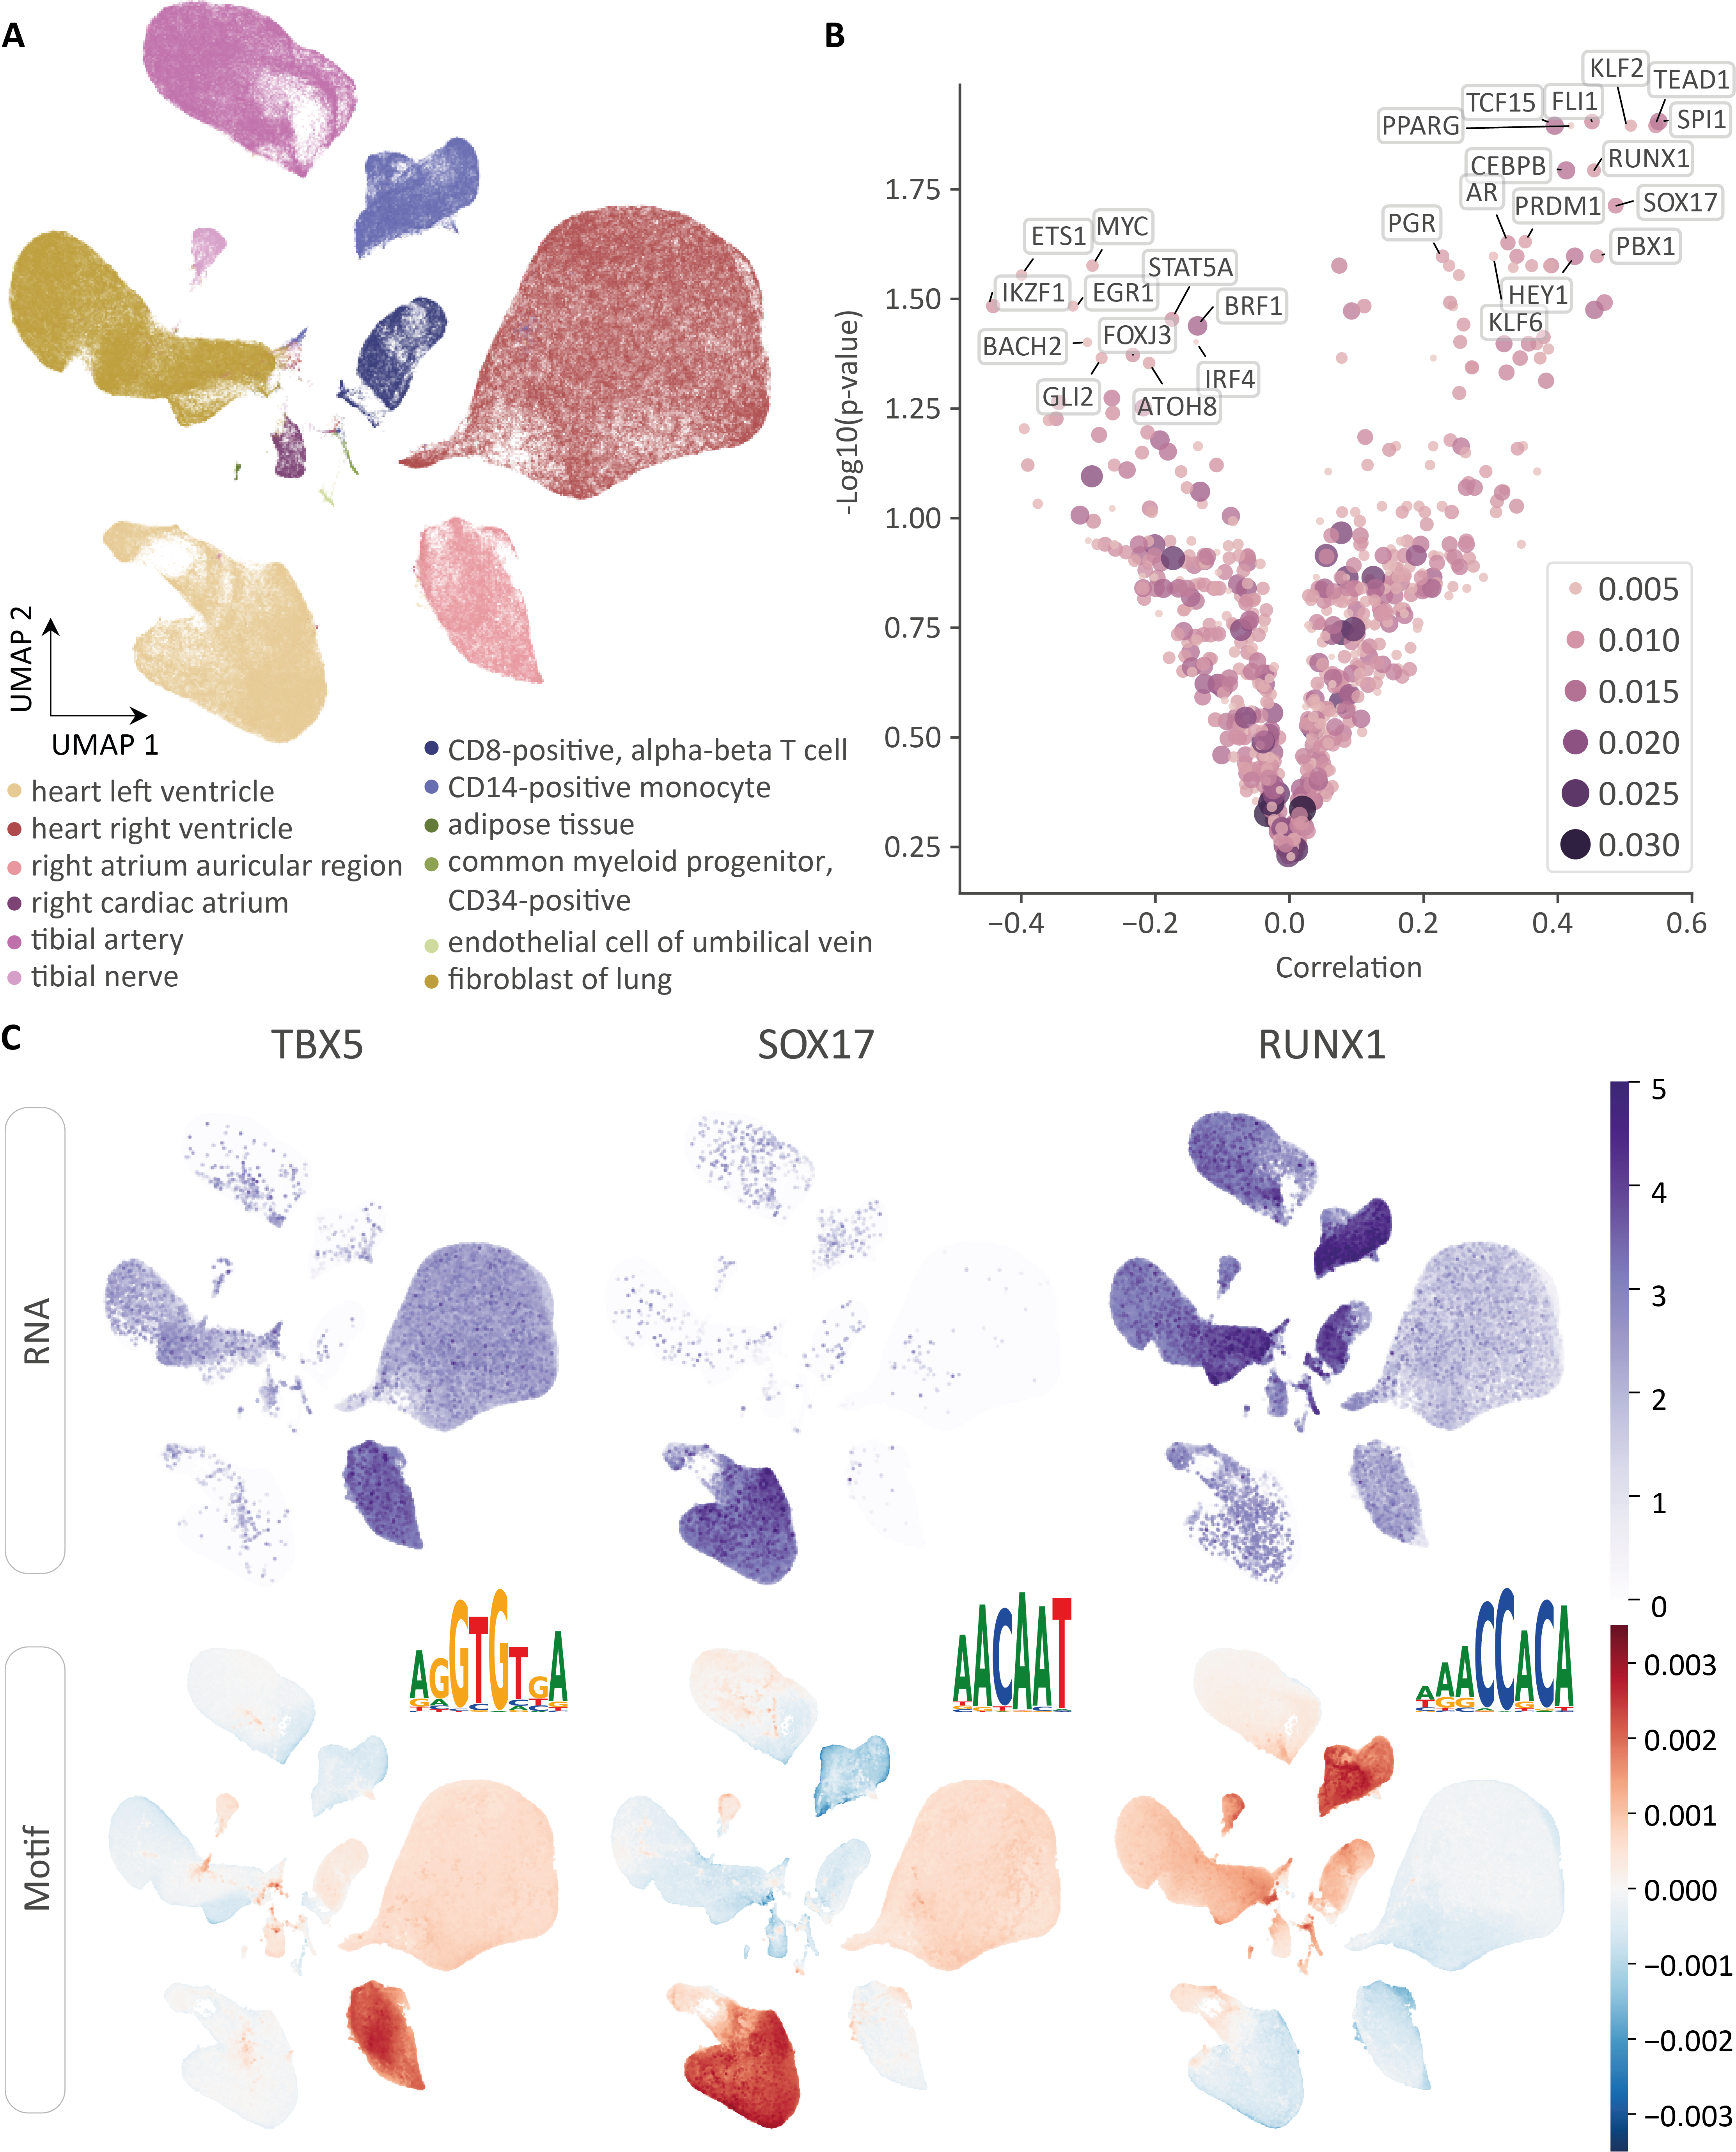
\includegraphics[width=0.75\linewidth]{SCEPIA_allCells_Fig1_v8_Calibri.png}
    \caption{\textbf{Figure XX: SCEPIA run on the Human Heart Cell Atlas} (a) UMAP representation, based on UMAP coordinates provided by the authors (\cite{Kanemaru2023}), with cluster annotation labels as predicted by SCEPIA. (b) Volcano plot of SCEPIA hits, labels of the top 15 of both correlating as anti-correlating hits are indicated, based on p-adj < 0.05 values. Dot size and color labels are based on the motif score standard deviations.  (c) Expression levels (top) of 3 well-known markers, TBX5 (cardiomyocytes), SOX17 (endothelial cells), RUNX1 (blood cells), and their predicted motif [[scores/activity]] by SCEPIA (bottom), printed on the UMAP as shown in (a). Sequence logos of the binding motifs are indicated, with the GimmeMotifs database identifiers (left to right): GM.5.0.T-box.0005, GM.5.0.Sox.0021, GM.5.0.Runt.0003. }
    \label{fig:scepia_hhca1}
\end{figure}
TBX5 CM marker, SOX17 endothelial marker, RUNX1 lymphoid marker 

% \hvFloat[doublePage,capWidth=n,
% capPos=bottom,bindCorr=0.0cm]{figure}
% {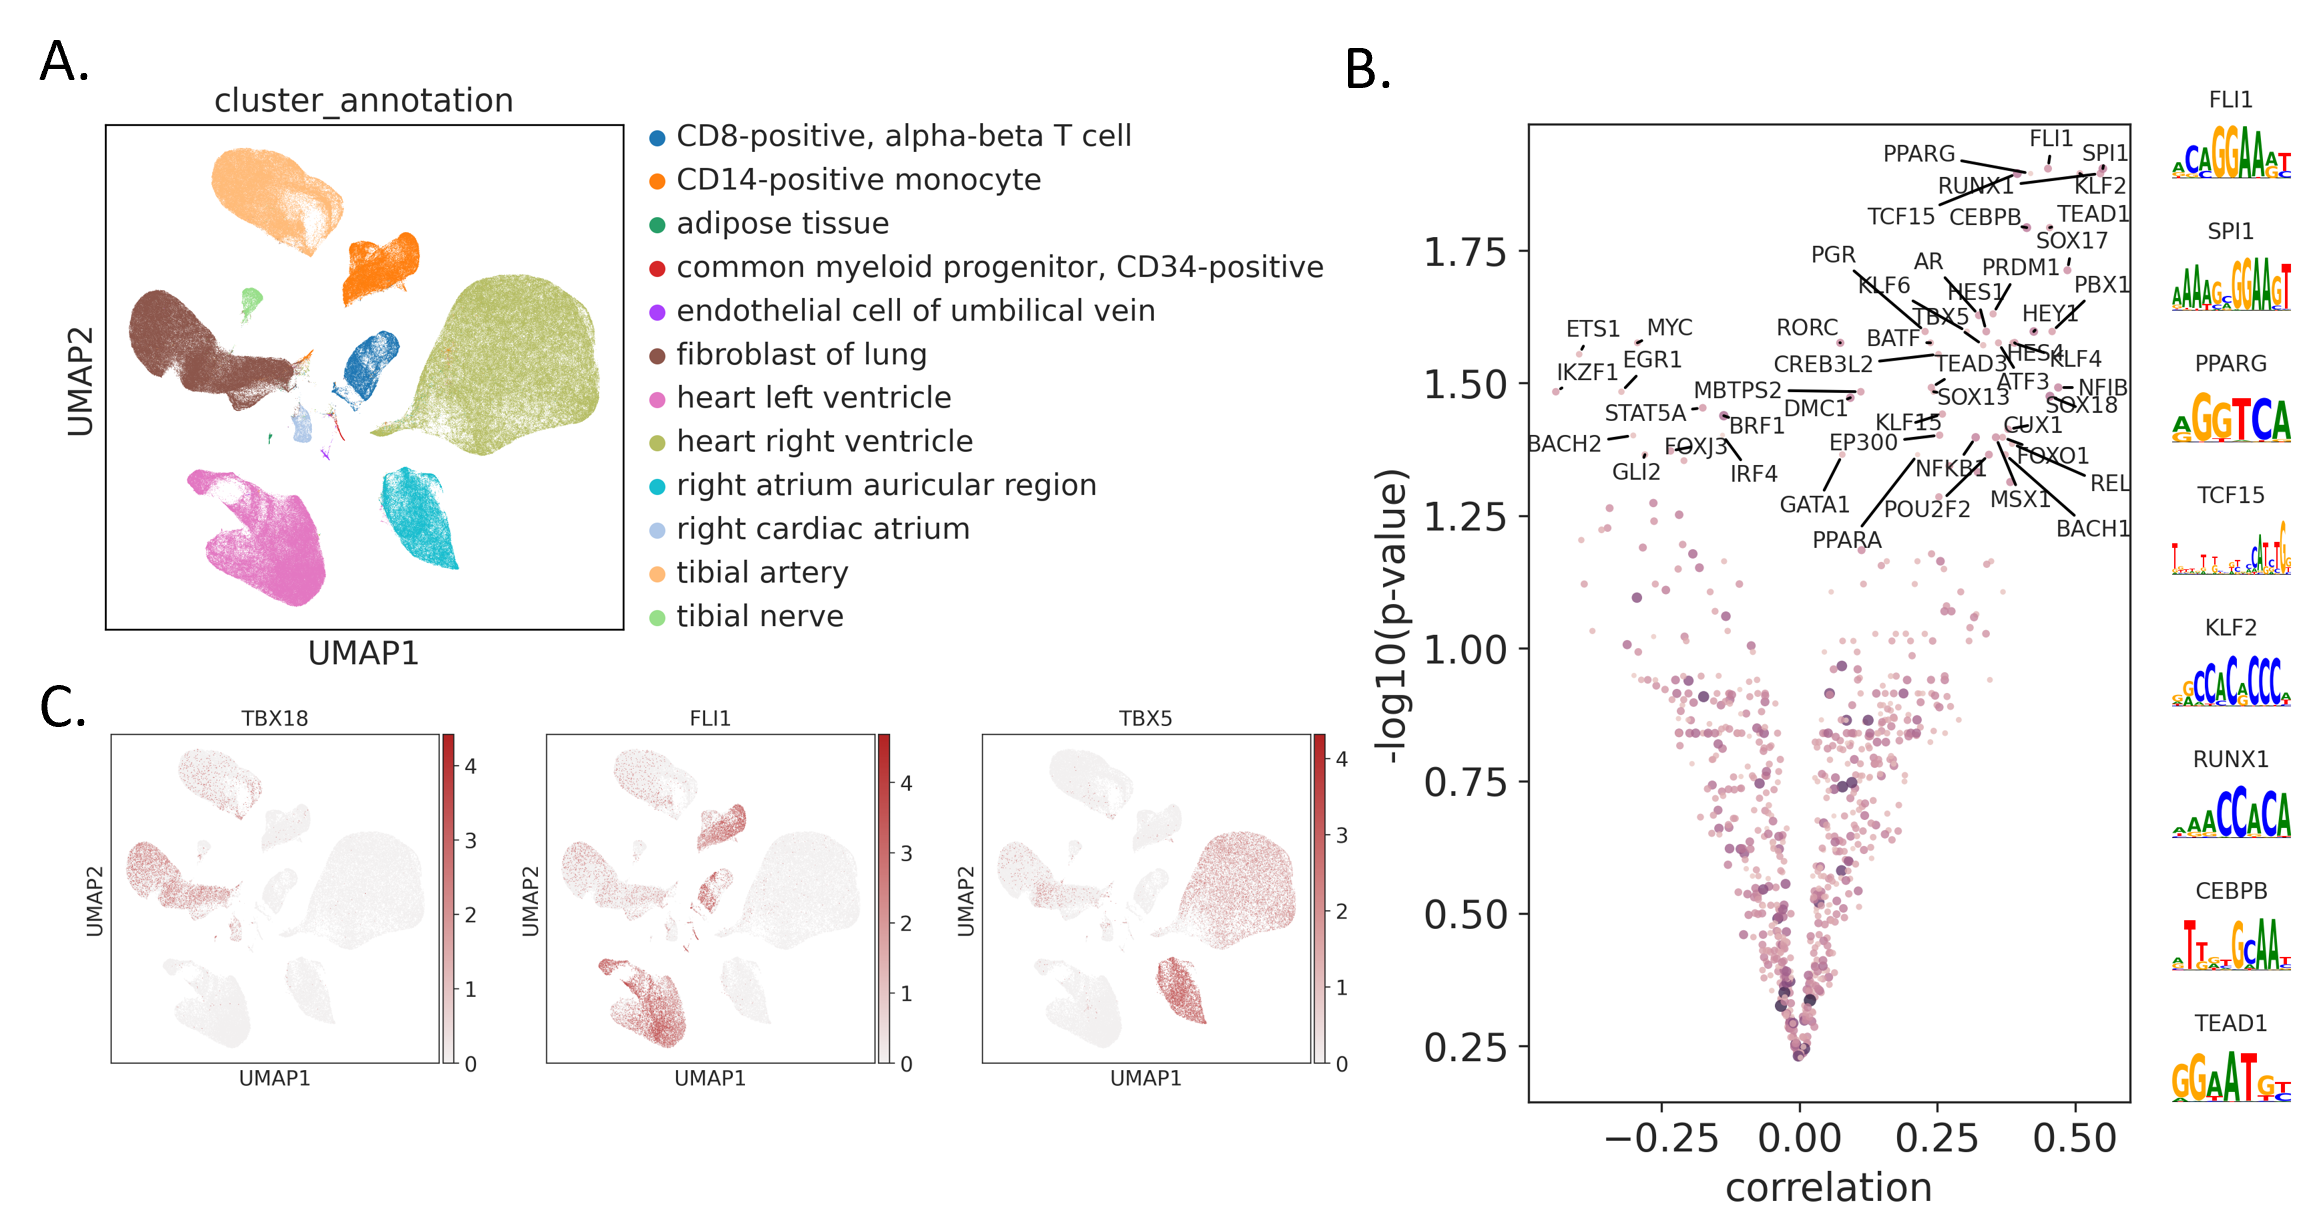
\includegraphics[width=1.6\textwidth]{ch.scepia/imgs/SCEPIAonHHCA.png}}
% [blabla]
% {SCEPIA run on the human heart cell atlast}{fig:scepia_hhca}

\begin{figure}
    \centering
    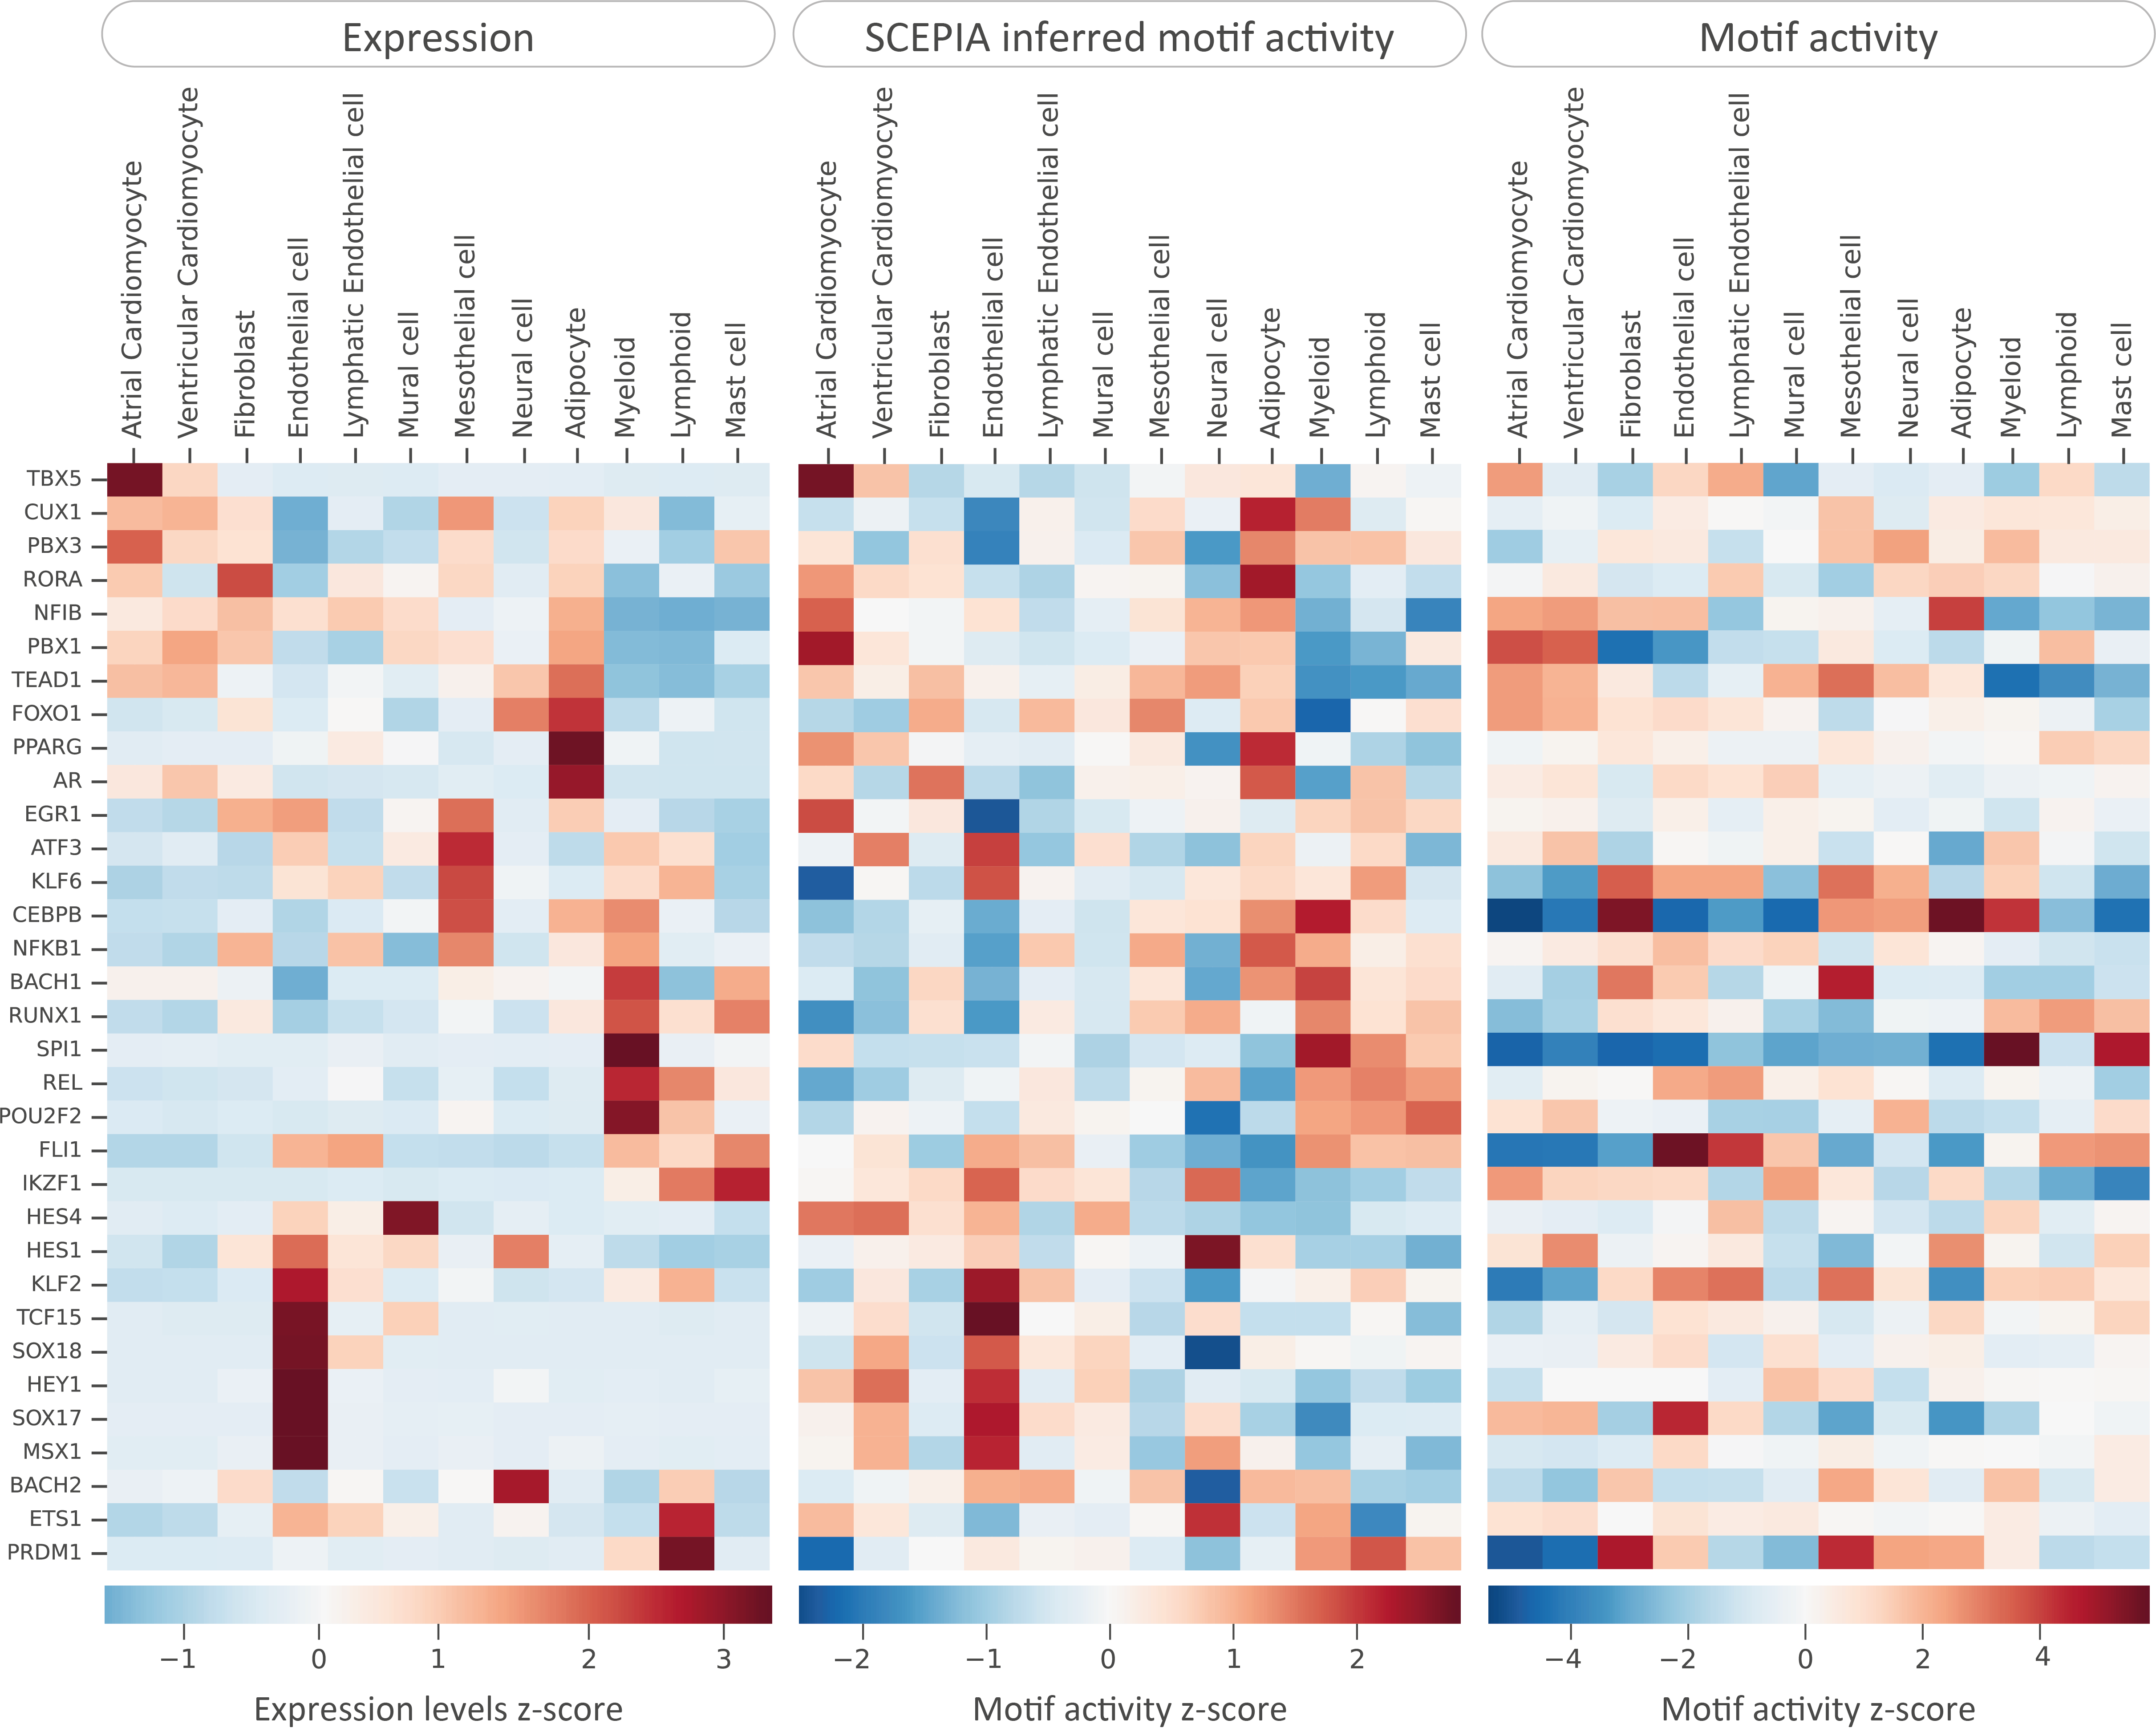
\includegraphics[width=0.75\linewidth]{SCEPIAhitsHHCA_HeatmapExprSCEPIAMaelstrom_v2.png}
    \caption{\textbf{Figure XX: Gene expression, SCEPIA and Maelstrom analysis on the human Heart Cell Atlas v2.} Significant transcription factor and binding motif hits (p-adj < 0.05) from the SCEPIA analysis on the human Heart Cell Atlas v2 were selected, and visualized as: Cluster averaged gene expression levels per transcription factor (left), cluster averaged motif activities for the predicted binding motifs inferred by SCEPIA from a H3K27Ac data reference (middle) and the motif activities as predicted by GimmeMotifs Maelstrom on the averaged scATAC-signal per cluster (right).}
    \label{fig:scepia_hhca2}
\end{figure}

Comparing SCEPIA with Maelstrom motif activities
For the interpretation of the motifs, it's also good to consider the difference between H3K27ac and accessibility. These assays measure different things. Nuclear receptor motif may not be necessarily associated with differential accessibility, if these factors bind in pre-existing accessible regions to regulate enhancer activity.
\textit{-> 1 large cluster of adipocyte expressed factors (RORA-[...]-AR) that have no expression in the immune cell types (Myeloid, Lymphoid, Mast cell), show an irregular pattern of accessibility in the ATAC data for the immune cells. (OR the protein is still there and its not measured in the RNA levels) Combining the motif accessibility with the expression levels of their binding targets, shows a specificity of these factors for the adipocytes (and some in CM) which was not picked up in the maelstrom analysis.\href{https://www.cell.com/molecular-cell/fulltext/S1097-2765(00)80209-9?_returnURL=https\%3A\%2F\%2Flinkinghub.elsevier.com\%2Fretrieve\%2Fpii\%2FS1097276500802099\%3Fshowall\%3Dtrue}{PPAR gamma is required for placental, cardiac, and adipose tissue development }}
-> CEBPB does not belong in fibroblasts.
-> TBX5 is well-known marker for CM (not lymphatic)
BACH2 is known as a repressor, shows high expression in neural cell, associated with negative motif activity
- it seems mural and mesothelial cells show relatively low motif activities (either positive or negative). Could suggest that here not enough matching H3K27ac cell types are available (they are probably not represented as pure cell types, and in tissue samples they're probably not abundant enough). Additionally, they are also not marked in the UMAP. Are they presen in very low numbers? In any case, enough explanations for why SCEPIA fails. Same cell types also perform the worst in the benchmark below).

\textbf{NEEDED FIGURE???}
SCEPIA on 100K subsets of HHCA scRNA-seq versus naive correlations between Maelstrom motif activity and binding gene expression levels
SCEPIA with and without geosketch filtering: \textbf{check for interesting biology} -> Otherwise \textit{maybe} supplemental.
\begin{figure}
    \centering
    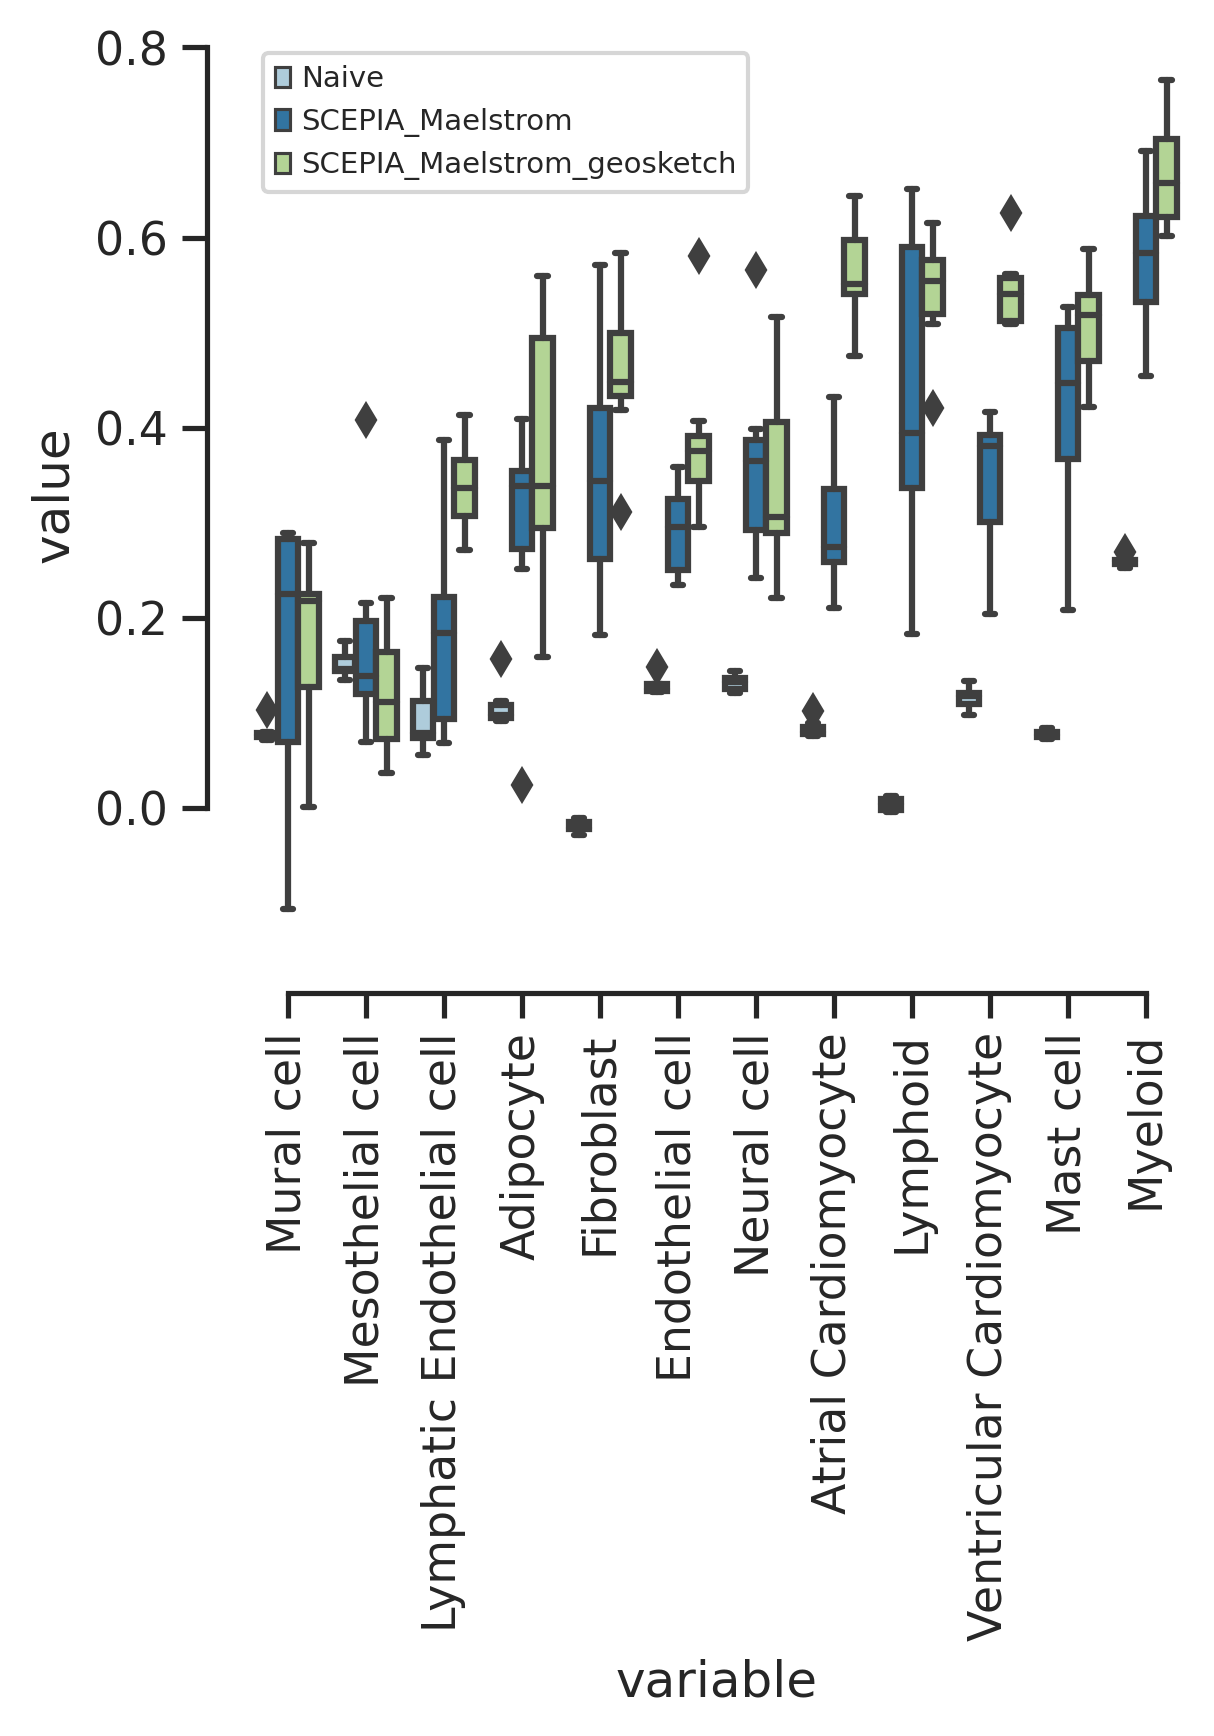
\includegraphics[width=0.75\linewidth]{ch.scepia/imgs/CorrelationsGeosketch_perCT.png}
    \caption{SCEPIA sc benchmark - Geosketch}
    \label{fig:sc_benchmark}
\end{figure}

\section{Discussion}

\subsection{Limitations}
\begin{itemize}
    \item Benchmark is bad. Benchmarking against a bad ground truth is stupid.
    \item Can not detect alternative splcing / rna degradation / post translational modificaitons etc.
    \item Why do we use ridge / lasso? Why not elasticnet?
\end{itemize}

\section{Methods}

\subsection{Overview of public data}

\subsubsection{Sequencing data}

Table RNA-seq
 96  RNA-seq cell types (accession + cell type)
 
 Table H3K27ac
 121 human H3K27ac cell types (Accession + cell type)

\subsubsection{Cis-regulatory regions}

We used a collection of cis-regulatory regions, based on all human transcription factor ChIP-seq peaks from ReMap 2018 (\href{http://remap.univ-amu.fr/storage/remap2018/hg38/MACS/remap2018_all_macs2_hg38_v1_2.bed.gz}{http://remap.univ-amu.fr/storage/remap2018/hg38/MACS/remap2018\_all\_macs2\_hg38\_v1\_2.bed.gz}) (\href{javascript:;}{41}), as described previously (ref ANANSE). This collection of enhancers is available at Zenodo with doi 10.5281/zenodo.4066423.

\subsubsection{Human heart cell atlas}

[Description]

\subsection{RNA-seq processing}

Preprocessing of RNA-seq was done automatically by seq2science v1.0.3 \cite{seq2science} using the rna-seq workflow. Public samples were downloaded from the Sequence Read Archive \cite{Leinonen2010} with help of the NCBI e-utilities and pysradb\cite{Choudhary2019}. Genome assembly GRCh38.p13 was downloaded with genomepy 0.16.1 \cite{Frlich2023}. Paired-end reads were trimmed with fastp v0.23.2 \cite{Chen2018} with default options. Reads were aligned with STAR v2.7.10b \cite{Dobin2012} with default options. Afterwards, duplicate reads were marked with Picard MarkDuplicates v3.0.0 \cite{picard}. BAM files were converted to CRAM format with samtools v1.16 \cite{Danecek2021}. Read counting and summarizing to gene-level was performed on filtered BAM files using HTSeq-count v2.0.2 \cite{Anders2014}. TPM-normalized gene counts were generated using genomepy based on longest transcript lengths.

\subsubsection{H3K27ac ChIP-seq processing}

Then align all human h3k27ac from ENCODE to remap peaks. qnorm \cite{qnorm}
[expand]

\subsection{Regulatory potential}

The cell type-specific regulatory potential[ref] P of gene $g$ is calculated similar to as:
        \begin{equation*}
            P_g = \sum_k w_{k}s_{k,g}
        \end{equation*}
        where $w_k$ is the weight at position $k$, and $s_{k,g}$ is the \textbf{log1p-transformed? TODO} h3k27ac signal at position $k$ for gene $g$.
        
The weight $w_k$ is calculated identically to ANANSE (ref):
        \begin{equation*}
            w_k = \begin{cases}
                1, & \text{if } k \in (0\,\text{kb},\ 5\,\text{kb}] \\
                \frac{2e^{-\mu|k-t_g|}}{1+e^{-\mu|k-t_g|}}, & \text{if } k \in (5\,\text{kb},\ 100\,\text{kb}]
            \end{cases}
        \end{equation*}
        where parameter $t_g$ is the genomic position of the TSS of gene $g$, and $\mu$ determines the decay rate as a function of distance from the TSS, set such that an enhancer 10 kb from the TSS contributes one-half of an enhancer within 5 kb from TSS. $t_g$ is the distance from the TSS.


\subsection{Regulatory motif analysis and motif and transcription factor activity}

In the regulatory potential benchmark (Fig XX) and in SCEPIA we use the \textbf{\textit{motif}} \textbf{\textit{activity}} as a measure of motif or transcription factor importance. The motif activity (ref MARA; ISMARA\cite{Balwierz2014}) is calculated using the Bayesian ridge regression implemented in gimmemotifs\cite{Bruse_2018}, with the motif log-odds scores as features and the H3K27ac signal as predictor variable. In short, for each each region cis-regulatory region in the input we compute the motif log-odds score for each motif in the gimmemotifs database (gimme.vertebrate.XX). This motif databases contains a non-redundant collection of vertebrate transcription factor motifs\cite{Bruse_2018}. We assume that the H3K27ac signal in each enhancer, expressed as log2(# of reads + 1), is the sum of all motif log-odds scores multiplied by their respective motif weights. We then estimated these motif weights using lasso regression, where the regularization parameter ($\lambda$) was determined through 5-fold cross-validation. These motif weights, the feature coefficients from the fitted regression model, are used as a measure of motif importance, the motif activity. This measure can than be used as \textit{\textbf{transcription factor activity,}} based on the TFs that are predicted to bind to the motif.

\subsection{Benchmark of regulatory potential-based cell type and motif assignemt.}

To assess the performance of the regulatory potential-based approach compared to the actual H3K27ac signal, we conducted a systematic analysis. Our approach involved data subsampling and calculating correlation coefficients to evaluate the relationship between the ground truth data and the regulatory potential-based approach. Specifically, this analysis utilized two data sources: the bulk H3K27ac reference database encompassing 121 tissues from ENCODE and 1,268,775 REMAP peaks, as well as the RNA-seq database featuring 96 tissues from ENCODE (Table SX).

To establish a ground truth for comparison, we calculated the motif activity using the top 25,000 enhancers with the highest coefficient of variation with GimmeMotifs version XX \cite{Bruse_2018}. We selected random subsets of five tissues from X tissues shared between the RNA-seq database and the H3K27ac reference database.  The motifs were assigned to TFs, and we calculated the Pearson/Spearman correlation coefficients between the estimated motif activity and the ground truth motif activity for each tissue in each comparison.

In a naive approach to estimating motif scores, we consider the transcripts per million (TPM) of a transcription factor directly as the motif score. When multiple transcription factors are associated with a single motif, we use their mean.

In the regulatory potential-based approach, we exclude the five ground truth tissues from the reference database. We then convert the H3K27ac signal from the reference database into regulatory potential and subsequently perform regression analysis against the TPM values. This results in a 5 x XYZ table of regression weights. We select the top 50 tissues with the highest absolute regression weights and identify the top 10,000 differential enhancers between them. We then conduct a motif scan similar to the one performed for the ground truth, regressing the H3K27ac signal with the motif scores in these enhancers. Finally, the motif scores for our original five tissues are calculated by taking the dot product of the motif scores in the top 50 tissues and the tissue weights.

To assess the impact of using only the top 10,000 peaks for the regulatory-based approach while retaining the top 25,000 peaks for the ground truth, we also compute motif scores based on the top 10,000 differential enhancers (again selected based on coefficient of variation).

This entire process was repeated one hundred times to generate a distribution of correlation coefficients, providing an estimate of each approach's performance.

\subsection{Scepia}

The single-cell regulatory-based approach (scepia) is similar to the bulk approach. However, due to the enormous increase in data, some steps need to be altered from a computational resource point of view. In addition, the fact that a single-cell dataset usually consists of multiple related cell types, with a more fluent gradient in gene expression and thus motif scores, makes it so that this information can be used to infer "significantly" differential transcription factors based on motif scores and gene expression data.

\noindent
Required input:

\begin{itemize}
	\item Reference database matrix of peak intensities (D) with dimensions (peaks x cell types). Scepia comes with multiple extensive reference databases, and the user does not need to provide them themselves. These reference databases can be extended however.
    \begin{itemize}
    \item The peaks are based on REMAP, and consist of 1,268,775 putative enhancers.
    \item The different cell types from ENCODE, consisting of X tissue types.
    \item The values are the quantile normalized log1p (\textbf{IS THIS TRUE?}) counts.
    \item Most reference databases are based on H3K27ac signal, but this can be any chromatin mark associated transcription, for example, ATAC-seq.
    \end{itemize}
	\item Single-cell RNA-seq dataset S with dimensions (cells x genes). 
    \begin{itemize}
        \item ...?
    \end{itemize}
\end{itemize}

\noindent
Single-cell epigenome-based inference of activity can be divided into five main steps (see fig. \ref{fig:scepia_overview}):

\begin{enumerate}
    \item \textbf{Conversion of Reference Database Matrix}:
    
    Convert the reference database matrix of peak intensities $D$ into a database matrix of regulatory potential per gene $P$ with dimensions $(\text{genes} \times \text{cell types})$. The reference database includes all REMAP peaks, including promoters, and is prepared beforehand.
    
    \begin{itemize}
        \item The regulatory potential P of gene $g$ is calculated as:
        \begin{equation*}
            P_g = \sum_k w_{k}s_{k,g}
        \end{equation*}
        where $w_k$ is the weight at position $k$, and $s_{k,g}$ is the \textbf{log1p-transformed? TODO} h3k27ac signal at position $k$ for gene $g$.
        
        \item The weight function is calculated identically to ANANSE:
        \begin{equation*}
            w_k = \begin{cases}
                1, & \text{if } k \in (0\,\text{kb},\ 5\,\text{kb}] \\
                \frac{2e^{-\mu|k-t_g|}}{1+e^{-\mu|k-t_g|}}, & \text{if } k \in (5\,\text{kb},\ 100\,\text{kb}]
            \end{cases}
        \end{equation*}
        where parameter $t_g$ is the genomic position of the TSS of gene $g$, and $\mu$ determines the decay rate as a function of distance from the TSS, set such that an enhancer 10 kb from the TSS contributes one-half of an enhancer within 5 kb from TSS. $t_g$ is the distance from the TSS.
    \end{itemize}

    \item \textbf{Cell Annotation from Single-Cell Dataset}:
    
    Match cells in the single-cell dataset $S$ with regulatory potential $P$, resulting in an annotation matrix $A$ with dimensions $(\text{cells} \times \text{cell types})$. The transcript counts of each cell are regressed against the regulatory potential database (TODO, is x regressed against y, or vice versa?). The annotation matrix represents the regression coefficients, and cells receive a tissue/cell type annotation based on the highest regression coefficient.
    
    \begin{itemize}
        \item The first step involves selecting a subset of relevant cell types to speed up the cell annotation. It assumes that the user has already performed Louvain or Leiden clustering, and average counts are obtained per cluster. The top 2,000 most variable genes (dispersion normalized) are chosen. For each cluster $c$, the regression coefficients are calculated by lasso regression:
        % S_c = P A_c + \lambda ||A_c|| + \epsilon
        \begin{equation*}
            \underset{A_c}{\operatorname{argmin}}\ |S_c - P A_c| + \lambda |A_c|
        \end{equation*}

        Where the regularization parameter ($\lambda$) is estimated through 5-fold cross-validation.

        Absolute regression weights are summed per tissue/cell type, and only the (absolute) top 50 cell types/tissues are retained in the regulatory potential database.
        
        \item Mean center the single-cell counts and set each cell as the mean expression value of its neighbors. \textbf{TODO}, why no mean centering for regulatory potential? For each cell $i$, the regression coefficients are calculated using Bayesian ridge regression with the top 50 cluster weights:

        \begin{equation*}
            \underset{A_i}{\operatorname{argmin}}\ |S_i - P A_i|^2 + \lambda |A_i|^2
        \end{equation*}
        
        \item Cells are initially assigned the cell type/tissue with the highest weight, and clusters are annotated based on the most common cell type in that cluster. Cell types are further refined by taking the dot product of cell type weights with neighborhood weights. Cell types require a minimum of 50 cells for assignment; otherwise, they are labeled as "other."
    \end{itemize}

    \item \textbf{Motif Scan over Differential Enhancers}:
    
    Look up the H3K27ac signal of the annotated cell types and retain the top 10,000 enhancers with the highest variance between them. The resulting matrix is denoted as $E$ and has dimensions (10,000 x 1). Conduct a (differential) motif scan over these enhancers. 
    
    \begin{itemize}
        \item Only known motifs are considered. The gimmemotifs vertebrate motif database is used as default.
        \item For each enhancer, calculate the motif score (\textbf{how to call the motif score from scanning?)} by scanning the motif in the enhancer. The result is a matrix $O$ with dimensions (10,000 x nr of motifs).
        \item Motif weights ($M$) are calculated by Bayesian ridge regression:
        \begin{equation*}
            \underset{M}{\operatorname{argmin}}\ |E - O M|^2 + \lambda |M|^2
        \end{equation*}

        where the $M$ has dimensions (1 x nr of motifs).

        TODO check dimensions!

        \textbf{TODO}, the mean is subtracted here and I don't think it does anything meaningful... 
    \end{itemize}
    

    \item \textbf{Calculation of Motif Scores}:
    
    Calculate the motif scores for the cells based on the motif scores of the reference top tissues. The motif scores per cell are calculated as a dot product of the cell type annotation weight and motif scores per reference tissue / cell type.
    \begin{equation*}
        F = M \cdot A
    \end{equation*}
    TODO check dimensions!

    \item \textbf{Correlation Analysis of Motif and Transcript Scores}:
    
    Determine significant combinations by correlating motif scores ($F$) and transcript scores ($S$) between cells:
    \begin{itemize}
        \item Calculate the correlation coefficient between motif score and transcript counts.
        \item Randomly shuffle motif scores and calculate their correlation with transcript counts. Repeat this 100,000 times to obtain a distribution of correlation coefficients.
        \item Estimate two different p-values per TF-motif combination from this analysis: one based on the correlation coefficient relative to the total permuted set and another using only the permuted set of motif correlations. Combine these p-values using Fisher's method.
        \item Calculate motif activity by fitting a Gaussian mixture model with two components over the motif activity scores. These components represent "high" and "low" motif scores. Motif activity is computed as the probability that a motif score belongs to the "high" expressed group, and is thus constrained to the range of 0 to 1.
    \end{itemize}
\end{enumerate}

\subsection{Human Heart Cell atlas Single-cell comparison}
\textbf{Human Heart Cell Atlas single-cell comparison }
- We have used the full global log-normalised counts-containing h5ad object of the human Heart Cell Atlas v2 (HCA) project as provided by the authors (\cite{Kanemaru2023}), and preprocessed the data with Scanpy (v1.9.2). 
- Clustering and UMAP-embeddings were used as provided by the authors.
- The dataset was subsetted to contain only highly variable genes (selected using the default settings within Scanpy; "min_mean = 0.0125, max_mean = 3, min_disp = 0.5") and the normalized counts were scaled. 
- Both the neighborhood connectivities of the single cells, as well as PCA were rerun, as necessary input for SCEPIA. 
- SCEPIA's infer_motifs was run on the preprocessed data with the following settings: using the top 2000 highly variable genes, the top 10,000 most variable enhancers and a maximum of 50 cell types from the reference, ridge regression was used for motif activity analysis and no subsetting on the number of cells was performed (\textit{XX this I removed from the installation v0.5.1 -> not sure if this will be incoorporated in SCEPIA? XX}). 
- The ENCODE H3K27Ac human reference dataset and gimme.vertebrate.v5.0.pfm motif file from the GimmeMotifs were used as input. 
- The resulting data was visualized with seaborn v0.12.2, matplotlib v3.8.0 and gimme logo from GimmeMotifs (v0.18.0)

- To establish how reproducible the SCEPIA runs are, and to benchmark the results by comparing with Maelstrom analysis, we generated multiple \textit{exclusive (other word..XX)} subsets from the HCA. The scRNA-seq dataset was subsetted into seven datasets of 100,000 cells each, selected randomly over the whole dataset. Each of these subsets was preprocessed, by selecting and filtering on highly variable genes, scaling, selecting neighborhood connectivities and performing PCA analysis, as described above for the full dataset. Each of these subsets were used in seperate SCEPIA runs, also run with the same settings as above. 


\textbf{Motif scanning on scATAC-seq fraction of Heart Cell Atlas}
- The ATAC peak matrix object as provided by the authors, was normalized per cell for sequencing depth (multiplied by 10,000) and log1p transformed, the resulting dataset was averaged per cell type cluster.  
- Only peaks outside of promoter regions (2,000 bp up- and downstream of transcription start sites) were kept, to select for enhancer regions. 
- The top 200,000 most variable enhancers were selected and the z-scores per peak and across the cell type means were calculated.
- The scaled matrix was used as input for gimme maelstrom from the GimmeMotifs package (v0.18.0), the same motif position frequency matrix file as used in SCEPIA (gimme.vertebrate.v5.0.pfm), and hg38 as the reference genome. 
- XX SELECT MOTIFS OF INTEREST FROM THIS ANALYSIS: what z-score threshold was used XX

\textbf{\textit{"Benchmark"} SCEPIA with scATAC-seq motif analysis}
- For each of the seven scRNA-seq subsets of the HCA, the mean expression values per cell type were correlated with the mean motif scores per cell type of all its potential binding motifs, obtained from the Maelstrom analysis on the scATAC-seq data. This comparison is referred to as the Naive comparison. Only highly variable genes were selected for this analysis. 
- For the SCEPIA comparison, all significant hits from the analysis (p-adj < 0.05) were selected and the predicted motif activities averaged per cell type. These inferred cell type motif activities were correlated with the activities predicted by Maelstrom analysis for each cell type. 
- The correlations in all of these comparisons were performed using the Pearson correlation method.
 - GEOSKETCH? Include?

\section{Supplementals}
\beginsupplement
\begin{table}
    \begin{center}
        \begin{tabular}{||c c c c||} 
        \hline
        Weight curve & Correlation between & Correct specific & Correct broad \\[0.5ex] 
        \hline
        Ananse & $0.53 \pm 0.14$ & $64\%$ & $77\%$ \\ 
        \hline
        Wang & $0.54 \pm 0.15 $ & $64\%$ & $75\%$ \\
        \hline
        Promoter (2kb) & $0.54 \pm 0.14$ & $66\%$ & $77\%$ \\
        \hline
        Enhancer & $0.43 \pm 0.14$ & $60\%$ & $72\%$ \\
        \hline
        Random & NaN & $2\%$ & $3\%$ \\
        \hline
        \end{tabular}
        \caption{Caption of my table.}
        \label{table:1}
    \end{center}
\end{table}

\begin{figure}
    \centering
    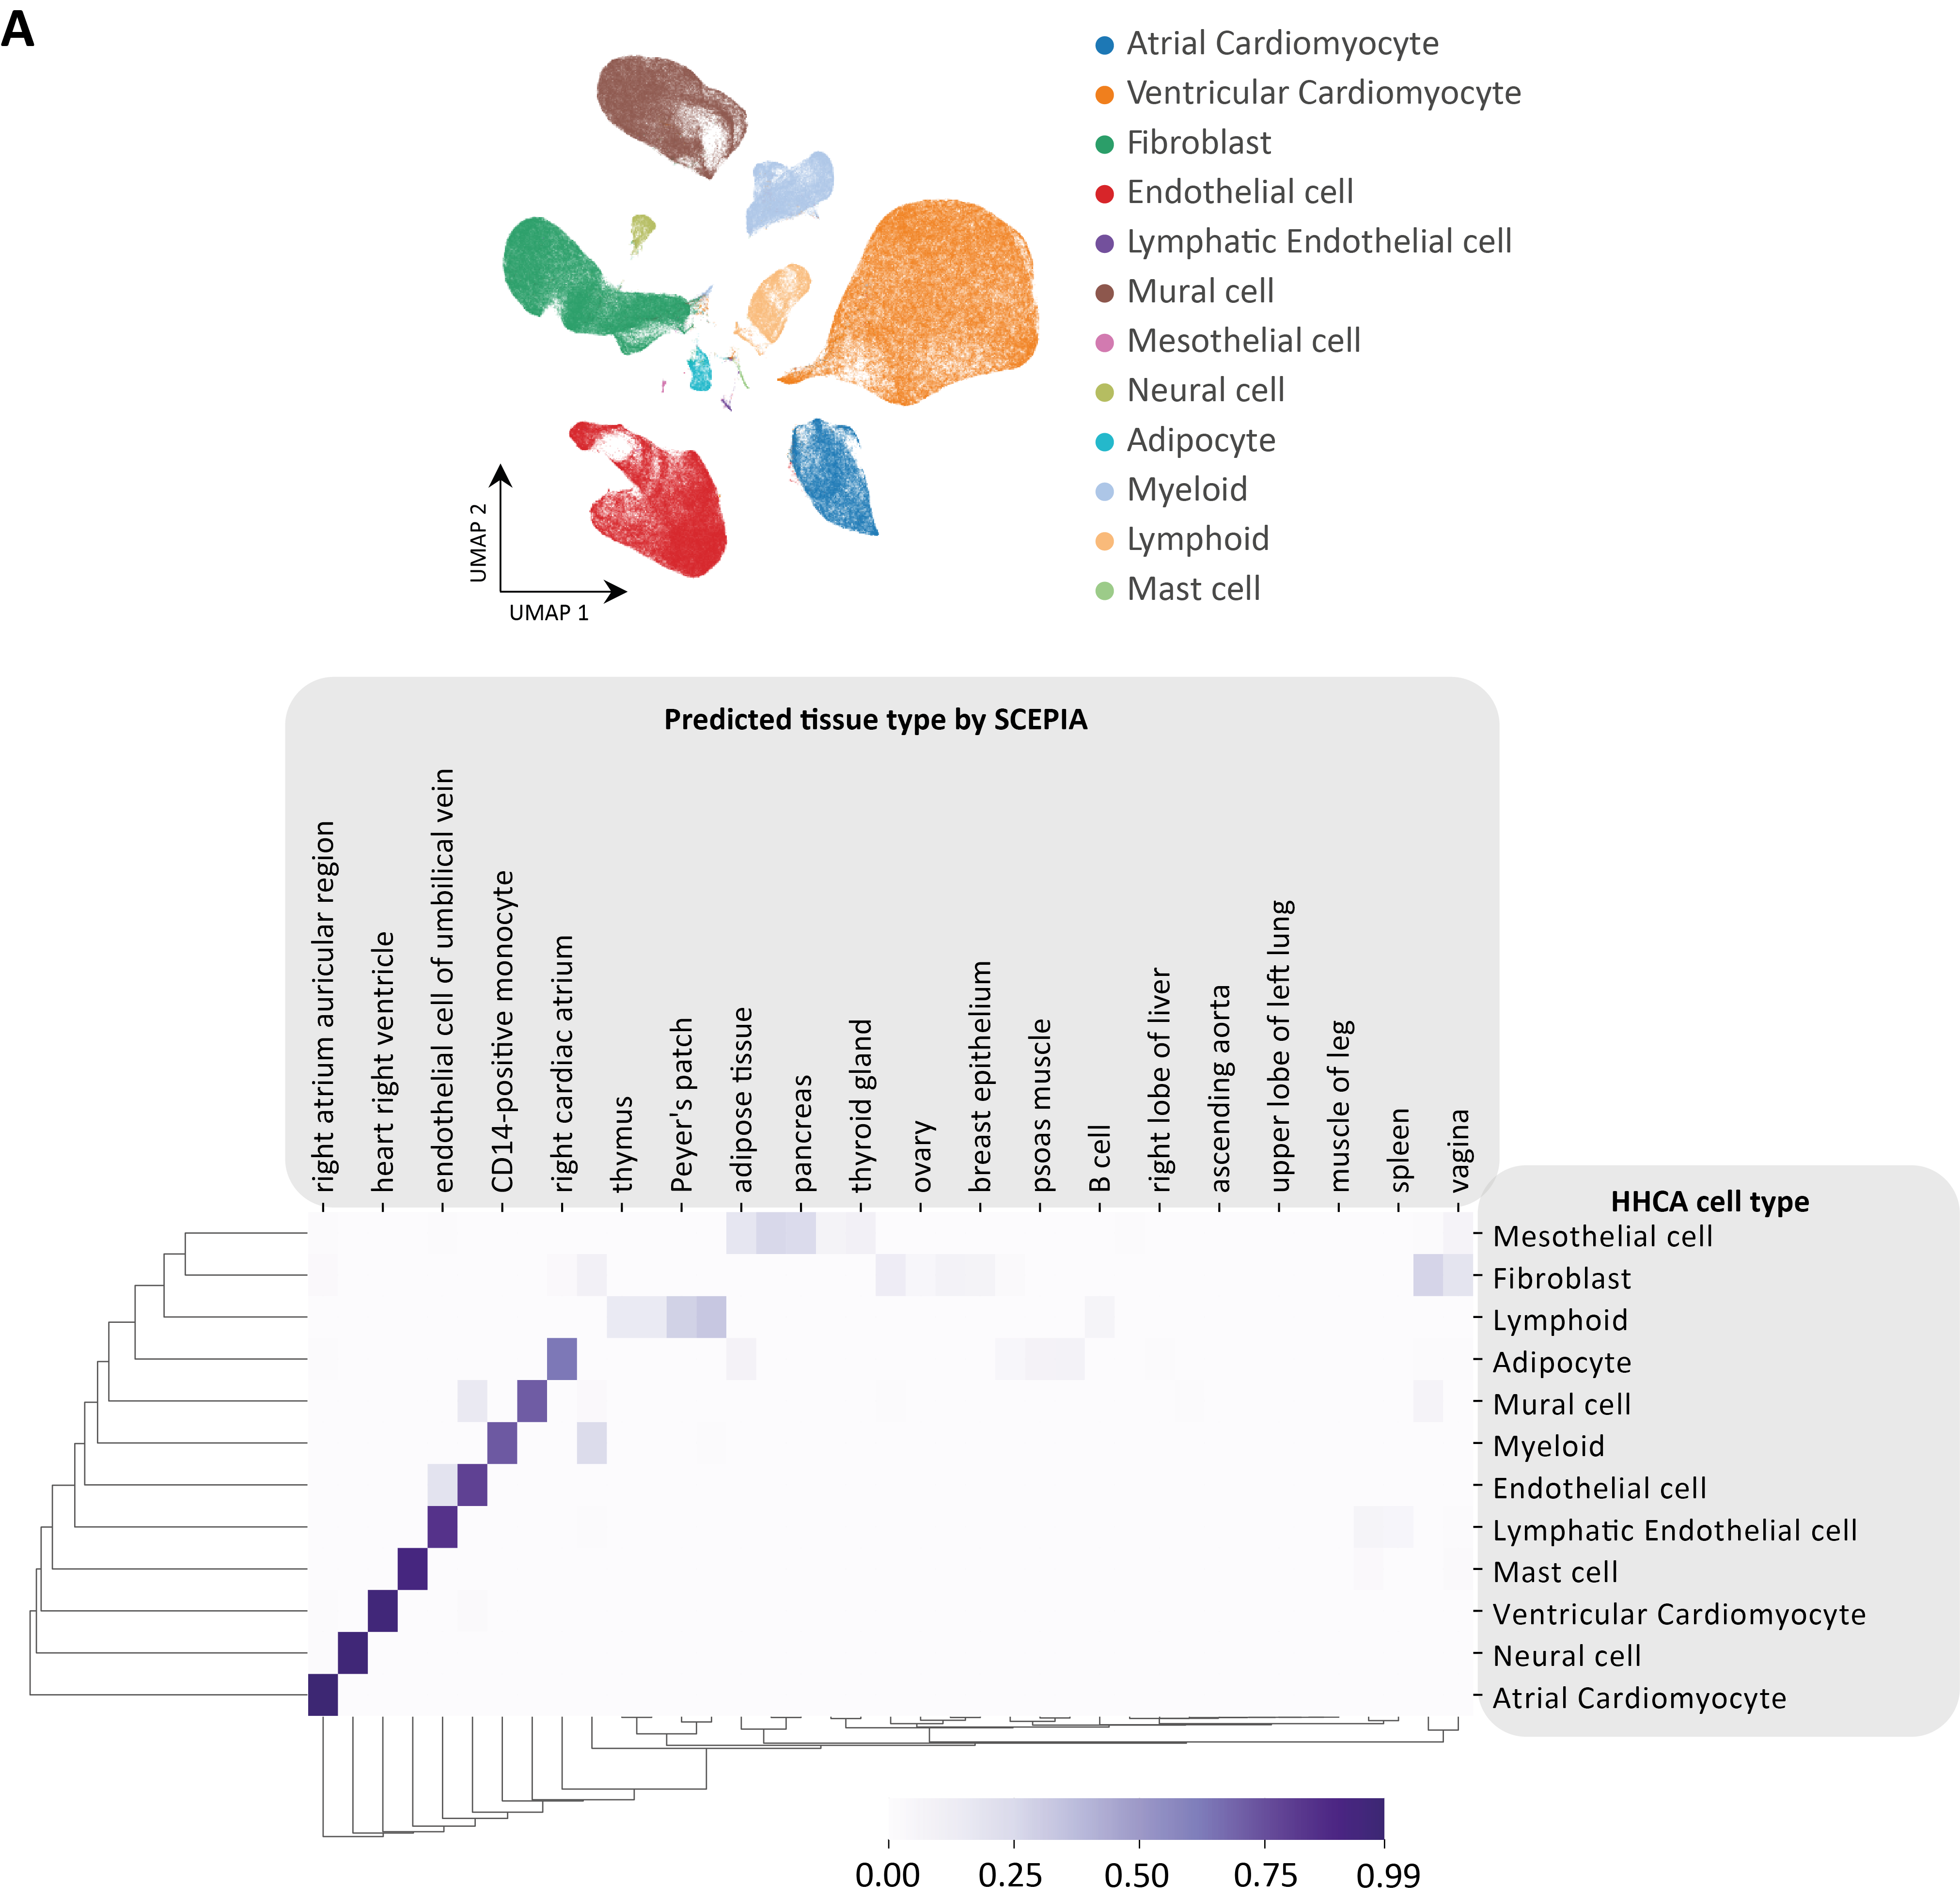
\includegraphics[width=\linewidth]{SCEPIA_Annotation_allCells_SuppFig1_v3.png}
    \caption{Original annotation of cell types (a) SCEPIA annotation of clusters (! Shit! It misses every other line in annotation of predicted TissueType!) (b) Highest scoring motifs inferred with SCEPIA run on 700K cells (placeholder) }
    \label{fig:scepia_hhca1}
\end{figure}